\chapter{Projeto Conceitual do Produto}

\section{Características gerais}

 O projeto do foguete tem como objetivo alcançar distâncias predefinidas de dez, vinte e trinta metros, com uma precisão de 0,5 metro, e que deve ser acionado eletromecanicamente à distância. Diante disso, o foguete deve ser reutilizado durante os três lançamentos, necessitando, assim, de uma estrutura consolidada e resistente, que assegure a firmeza da estrutura e proteja os componentes eletrônicos. O foguete será lançado a partir de uma base com ângulo fixo durante os três lançamentos. A partir disso, para a variação da distância, será necessário ajustar a pressão de lançamento. Sob esse viés, para o gerenciamento de todas essas necessidades, a equipe de eletrônica desenvolveu sistemas de armazenamento de dados e telemetria, capazes de registrar as informações necessárias para que os lançamentos cumpram os requisitos de projeto.

Ademais, a equipe de software desenvolveu algoritmos cruciais para o processamento dos dados coletados pelos sistemas eletrônicos, que permitem o ajuste da distância de lançamento. Também foi criada uma interface que possibilita a visualização dos dados do lançamento e dos sensores de forma simples e rápida. Portanto, com todos esses sistemas desenvolvidos, o foguete é capaz de suportar os lançamentos, além de fornecer visualizações digitais dos dados de maneira clara e acessível.

%\textcolor{red}{Descrever produto de forma geral. Apresentar itens teóricos sobre o projeto a serem aprofundados ou detalhados oportunamente.}

%\textcolor{red}{Apresentar e explicar a Estrutura Analítica do Projeto (EAP), tomando cuidado com a legibilidade da imagem. Se necessário, coloque a EAP dentro do comando ``\textsf{\textbackslash begin\{landscape\} \textbackslash end\{landscape\}}'' para que ela seja apresentada em uma página deitada.}

\begin{landscape}

\begin{figure}
    \centering
    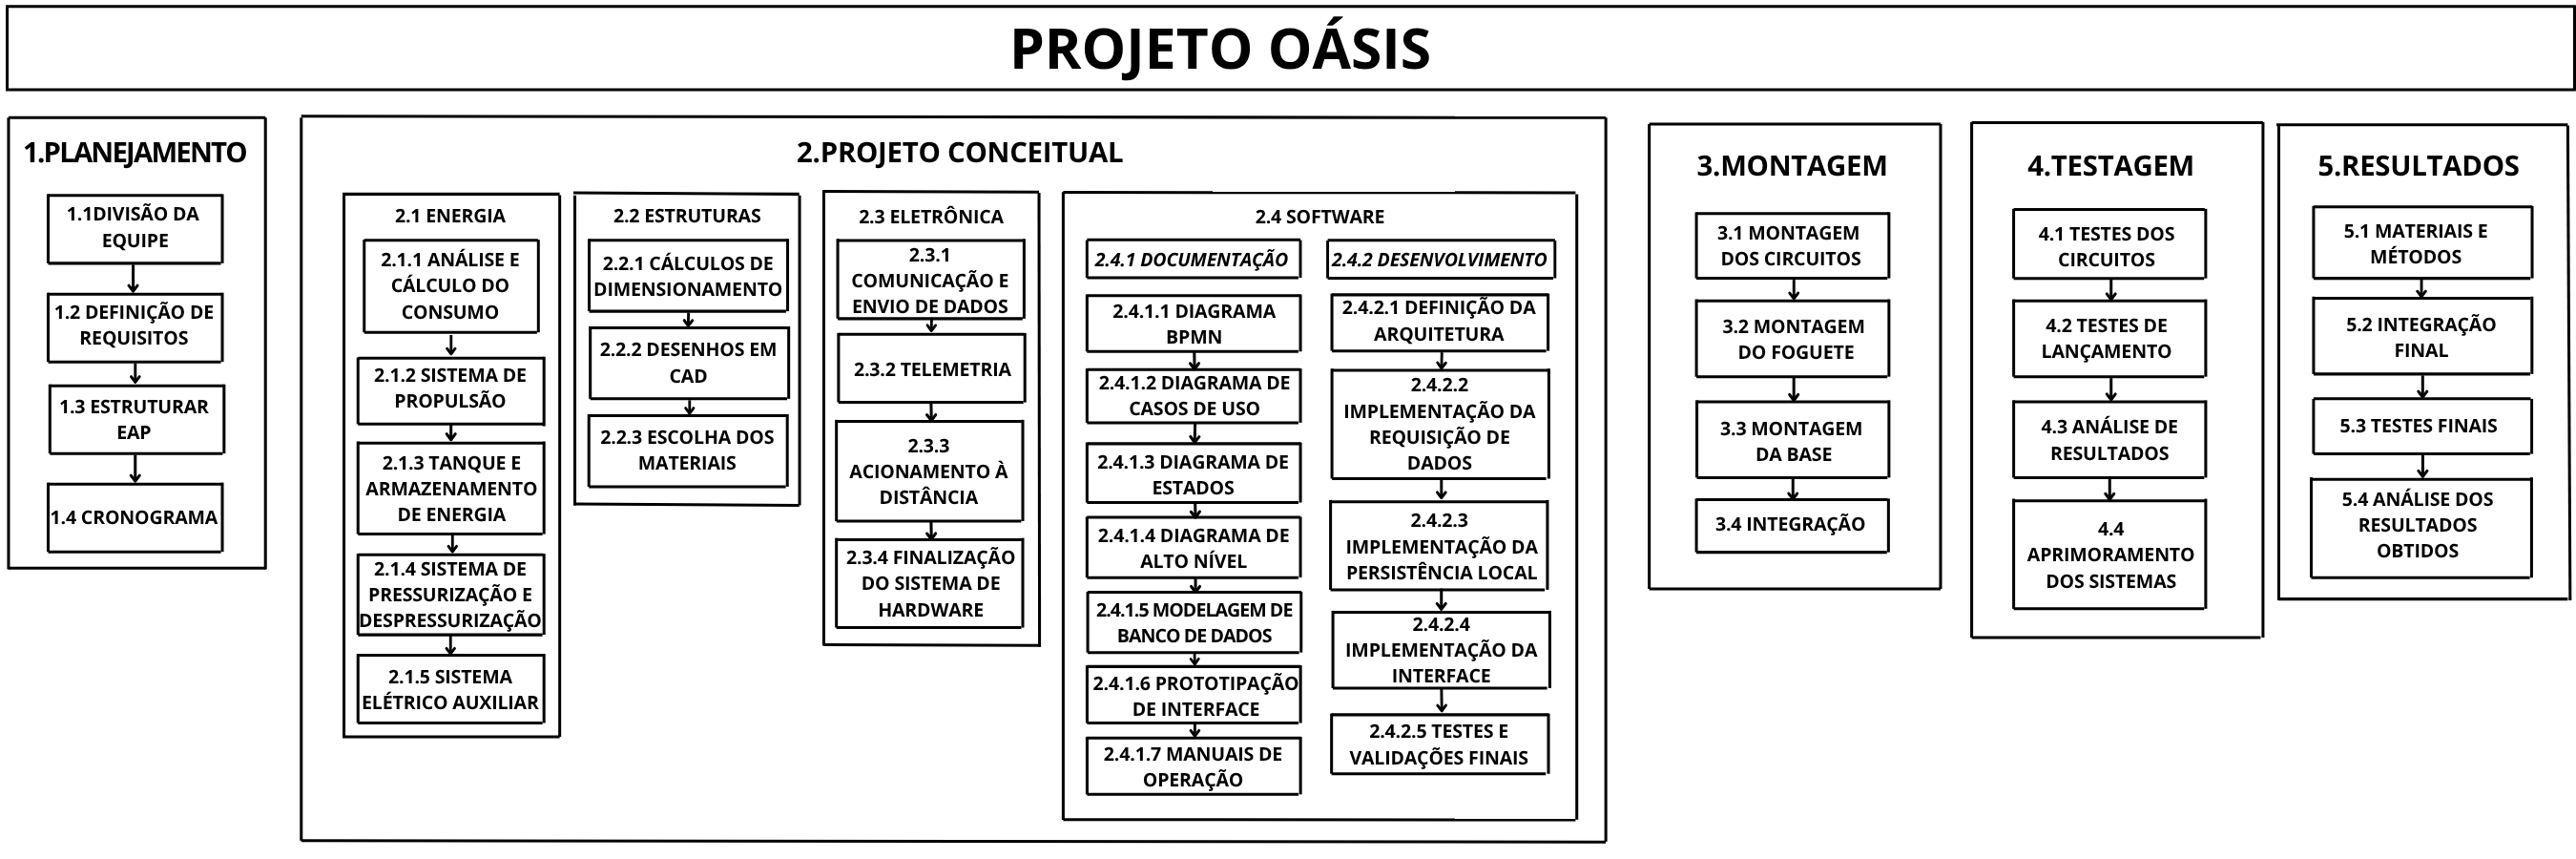
\includegraphics[width=1\linewidth]{figuras/EAP-corrigida.png}
    \caption{Estrutura analítica de projeto}
    \label{fig:enter-label}
\end{figure}

\end{landscape}

\section{Estrutura}

O projeto é composto por duas estruturas principais, o foguete, feito com garrafa PET, e a base de lançamento, construída com canos PVC sobre um painel de madeira. Assim, cada uma dessas partes tem funções e requisitos que devem ser cumpridos. 

Para o foguete, é necessário que ele seja feito de modo a suportar o abastecimento com água, a pressurização e três lançamentos consecutivos, sem se danificar e alcançando as distâncias exigidas. Dessa maneira, sua fabricação deve prezar pela resistência e pela aerodinâmica, a partir dos cálculos da trajetória.

Já a base de lançamento foi projetada considerando sua função de sustentar, pressurizar e lançar o foguete, colaborando para que ele cumpra seus requisitos. Além disso, ela deve ser capaz de medir a pressão dentro do foguete e de vedar o ponto de contato com ele.


\subsection{Escolha dos materiais}
A escolha dos materiais é uma das etapas mais importantes no desenvolvimento de qualquer projeto, pois influencia diretamente diversos aspectos fundamentais do resultado final. Entre os principais fatores impactados por essa decisão estão a resistência estrutural, a durabilidade, a segurança, a eficiência e a funcionalidade do item projetado. Além disso, a seleção adequada dos materiais pode otimizar o desempenho do produto em seu ambiente de uso, garantindo que ele atenda aos requisitos técnicos e operacionais esperados.

No nosso projeto, decidimos que o foguete seria construído utilizando uma garrafa PET de 1,5 litro, escolhida por ser leve, resistente à pressão e de fácil obtenção. Para garantir a estabilidade do voo, serão instaladas aletas, confeccionadas com um material leve e rígido (como papelão ou plástico), fixadas na parte inferior do corpo do foguete.

Já para sua base de lançamento, optamos por utilizar tubos de PVC de 32 mm, pois além de suportarem maiores pressões internas, estavam prontamente disponíveis, pois um dos membros do grupo já os possuía, o que reduziu o custo do projeto. No entanto, como o diâmetro de 32 mm não encaixava diretamente nas garrafas PET utilizadas como corpo do foguete, foi necessário utilizar adaptadores de 32 mm para 20 mm, além de segmentos de tubo de 20 mm. Também foram empregados conectores em “T” de 20 mm e 32 mm, além de tampas e outros acessórios, para permitir as conexões e direcionamentos do ar comprimido. Como o grupo definiu previamente que o foguete seria lançado com um ângulo fixo de 45°, utilizamos um joelho de PVC com essa mesma angulação para garantir essa inclinação de forma prática e estável. A estrutura foi firmemente fixada sobre uma placa de madeira com o auxílio de parafusos e abraçadeiras metálicas tipo U, garantindo estabilidade durante o lançamento. A câmara de pressão foi construída com um tubo de PVC de 32 mm, fechado por uma tampa na qual foi instalada uma válvula de bicicleta. Essa válvula permite a entrada de ar comprimido no sistema, proveniente de uma bomba de bicicleta. Para monitorar a pressão interna, foi instalado um manômetro acoplado por meio de um adaptador de 32 mm para rosca de ¼ de polegada, conectado a um redutor de ¼ para 1/8 de polegada.Para aumentar a segurança, incluímos um registro de 32 mm, utilizado como um mecanismo de alívio de pressão manual. Caso a pressão atinja níveis muito altos, o operador pode abrir o registro para liberar o ar e evitar danos à estrutura. Para assegurar a vedação do sistema e evitar qualquer vazamento de ar, utilizamos cola PVC e silicone em todas as conexão.

Portanto, é essencial que a seleção dos materiais sejam feita com base em uma análise criteriosa, levando em consideração fatores técnicos, e econômicos. A escolha consciente contribui para o sucesso do projeto, equilibrando desempenho, sustentabilidade e viabilidade financeira.



\subsection{Descrição do foguete}
O foguete Oasis será construído utilizando duas garrafas PET de 1,5 litros, que atuarão como reservatórios de ar e água, sendo responsáveis por gerar a força propulsora necessária para o lançamento. Para garantir maior estabilidade durante o voo, serão instaladas três aletas na parte traseira do foguete. Essas aletas poderão ser confeccionadas com materiais leves e resistentes, como plástico rígido reciclado ou papelão, visando um bom equilíbrio entre desempenho aerodinâmico e praticidade na fabricação.

Quanto ao sistema de propulsão, a garrafa será preenchida parcialmente com água, que atua como massa de reação no momento da ejeção. A proporção ideal entre água e ar foi determinada por meio de testes preliminares, visando maximizar os alcance delimintado proposto no projeto.
Todas as etapas de montagem será executadas com atenção à simetria, vedação e resistência estrutural,para garantir lançamentos seguros e eficientes. A tabela 2 detalha todos os materiais que provavelmente será empregados na construção do foguete.


%\begin{table}[htpb]
%\begin{center}
%\caption{Materiais usados no foguete}
%\begin{tabular}{|l|c|}
%\hline
%Garrafa PET 1,5L                     & 2 \\ 
%\hline
%Tubo de PVC 32mm                        &       \\ \hline
%Tubo de PVC 40mm                        &       \\ \hline
%\end{tabular}
%\end{center}
%\label{Tabela 2 - Materiais do Foguete}
%\end{table}

 \begin{figure}[H]
     \centering
     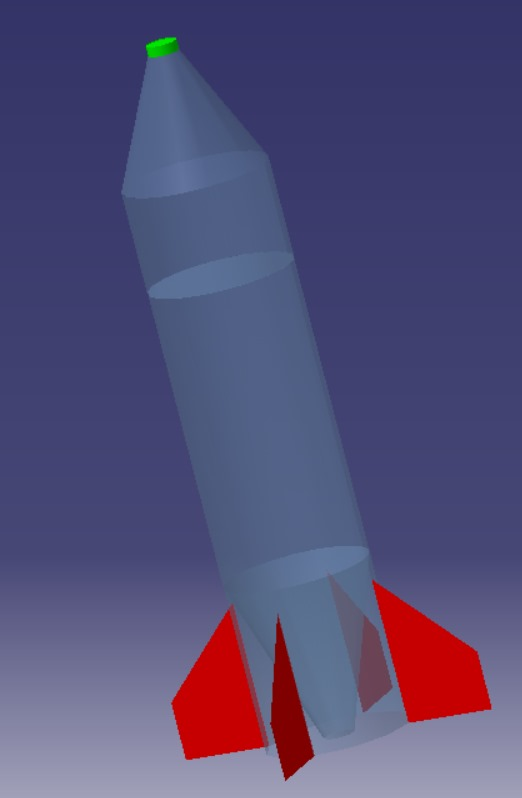
\includegraphics[width=0.30\textwidth]{figuras/cad foguete.jpg}
    \caption{CAD do foguete}
     \label{fig:tabela}
 \end{figure}


\subsection{Descrição da base de lançamento}

    A base do projeto Oásis foi desenvolvida com o objetivo de ser um suporte para o lançamento do foguete, permitindo a pressurização correta e fornecendo a angulação ideal para alcançar as distâncias previstas. A estrutura principal da base foi toda feita a partir de canos de PVC de 20 e de 32 milímetros de diâmetro, de acordo com a necessidade. No quesito da pressurização, a base foi equipada com uma válvula de bicicleta, para a entrada de ar, com um manômetro, para medir a pressão interna, e com um registro, que permite a liberação de pressão caso seja necessário. Dessa maneira, toda a estrutura da base será pressurizada, permitindo um controle mais acurado.
    
	Além disso, considerando que os lançamentos serão feitos todos a uma mesma angulação, foi garantida a precisão desta a partir do uso de um joelho de PVC de 45 graus. Ademais, para garantir a estabilidade da estrutura e do peso do foguete, o esqueleto de cano PVC foi parafusado a uma tábua de madeira com o uso de abraçadeiras de metal, o que garante a firmeza do sistema. Em conformidade com esse objetivo, foi adicionado um apoio ao suporte de lançamento, ligando-o também diretamente à placa de madeira. As quantidades dos materiais utilizados para a construção da base estão na Tabela 3.

\begin{table}[htpb]
\begin{center}
\caption{Materiais usados na base}
\begin{tabular}{|l|c|}
\hline
Tubo de PVC 20mm                        & 40 cm \\ \hline
Tubo de PVC 32mm                        & 32 cm  \\ \hline
Tubo de PVC 40mm                        & 5 cm  \\ \hline
Adaptador de PVC de 32mm para 20mm      & 2     \\ \hline
Adaptador de PVC de 32mm para ¼ pol     & 1     \\ \hline
Adaptador rosqueado de ¼ pol para 1/8 pol & 1   \\ \hline
Joelho de PVC de 32mm com 90°           & 3     \\ \hline
Joelho de PVC de 20mm com 45°           & 1     \\ \hline
Joelho de PVC em T 20mm                 & 1     \\ \hline
Joelho de PVC em T 32mm                 & 4     \\ \hline
Tampa de PVC 32mm                       & 1     \\ \hline
Registro de 32mm                        & 1     \\ \hline
Válvula de bicicleta                    & 1     \\ \hline
Manômetro                               & 1     \\ \hline
Fita veda-rosca                         & -     \\ \hline
Abraçadeiras de plástico                & 9     \\ \hline
Abraçadeira de metal circular           & 1     \\ \hline
Abraçadeira de metal tipo U             & 5     \\ \hline
Parafusos                               & 10    \\ \hline
Placa de madeira                        & 1     \\ \hline

\end{tabular}
\end{center}
\label{Tabela 3 - Materiais da Base de Lançamento}
\end{table}

%\pagebreak

 \begin{figure}[H]
     \centering
     \includegraphics[width=0.75\textwidth]{figuras/base de lançamento.jpg}
    \caption{Base de lançamento}
     \label{fig:tabela}
 \end{figure}

 \begin{figure}[H]
     \centering
     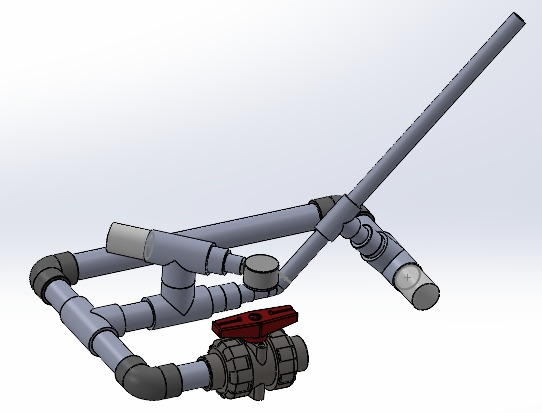
\includegraphics[width=0.5\textwidth]{figuras/cad da base.jpg}
    \caption{CAD da base}
     \label{fig:tabela}
 \end{figure}
 %\pagebreak
% \textcolor{red}{Apresentar desenho em CAD, indicar dimensões por lado/aresta/cota, indicar materiais utilizados e explicar o desenho e as decisões de projeto.}

 \section{Hardware}

 \subsection{Descrição de Hardware}

O diagrama de blocos ilustra a arquitetura do sistema, a lista de componentes foi selecionada para atender aos requisitos de telemetria e acionamento. O subsistema de telemetria é alimentado por uma fonte de 5V, que é regulada para 3.3V, suprindo energia ao sensor GPS NEO 6M 
e ao hardware microcontrolador ESP8266. O módulo GPS coleta dados de geolocalização e os envia ao ESP8266, que é responsável por processar e transmitir esses dados para um servidor de telemetria. De forma  independente, o subsistema eletromecânico opera com uma fonte de 12V  (bateria), alimentando diretamente o motor DC de 12V. O acionamento deste motor é efetuado por um botão “push”, indicando um controle de lançamento
manual e desacoplado do sistema de telemetria. O diagrama sistema de hardware proposto para o foguete de água compreende duas unidades principais: a Placa de Telemetria, embarcada no foguete, e a Placa de 
Acionamento, localizada na base de lançamento. A Placa de Telemetria é composta por um Módulo de Processamento e Comunicação (baseado no ESP8266), 
um Módulo GPS (ATK-NEO-6M) para aquisição de dados de voo, e um Subsistema de Alimentação (regulador AMS1117-3.3V e capacitores associados) para fornecer energia estabilizada aos componentes. A Placa de Acionamento integrará um Circuito de Interface com o Usuário (botão K4-6x6-TH), um Circuito de Pilotagem de Motor (transistor BD139, diodo 1N4001 e resistor de base) e o conector para o Motor DC12V, que efetuará o acionamento mecânico. As interligações essenciais incluem a comunicação serial entre o GPS e o ESP8266, a alimentação regulada para os módulos da telemetria, e o sinal do botão controlando o transistor que, por sua vez, aciona o motor.
 
 \begin{figure}[H]
    \centering
    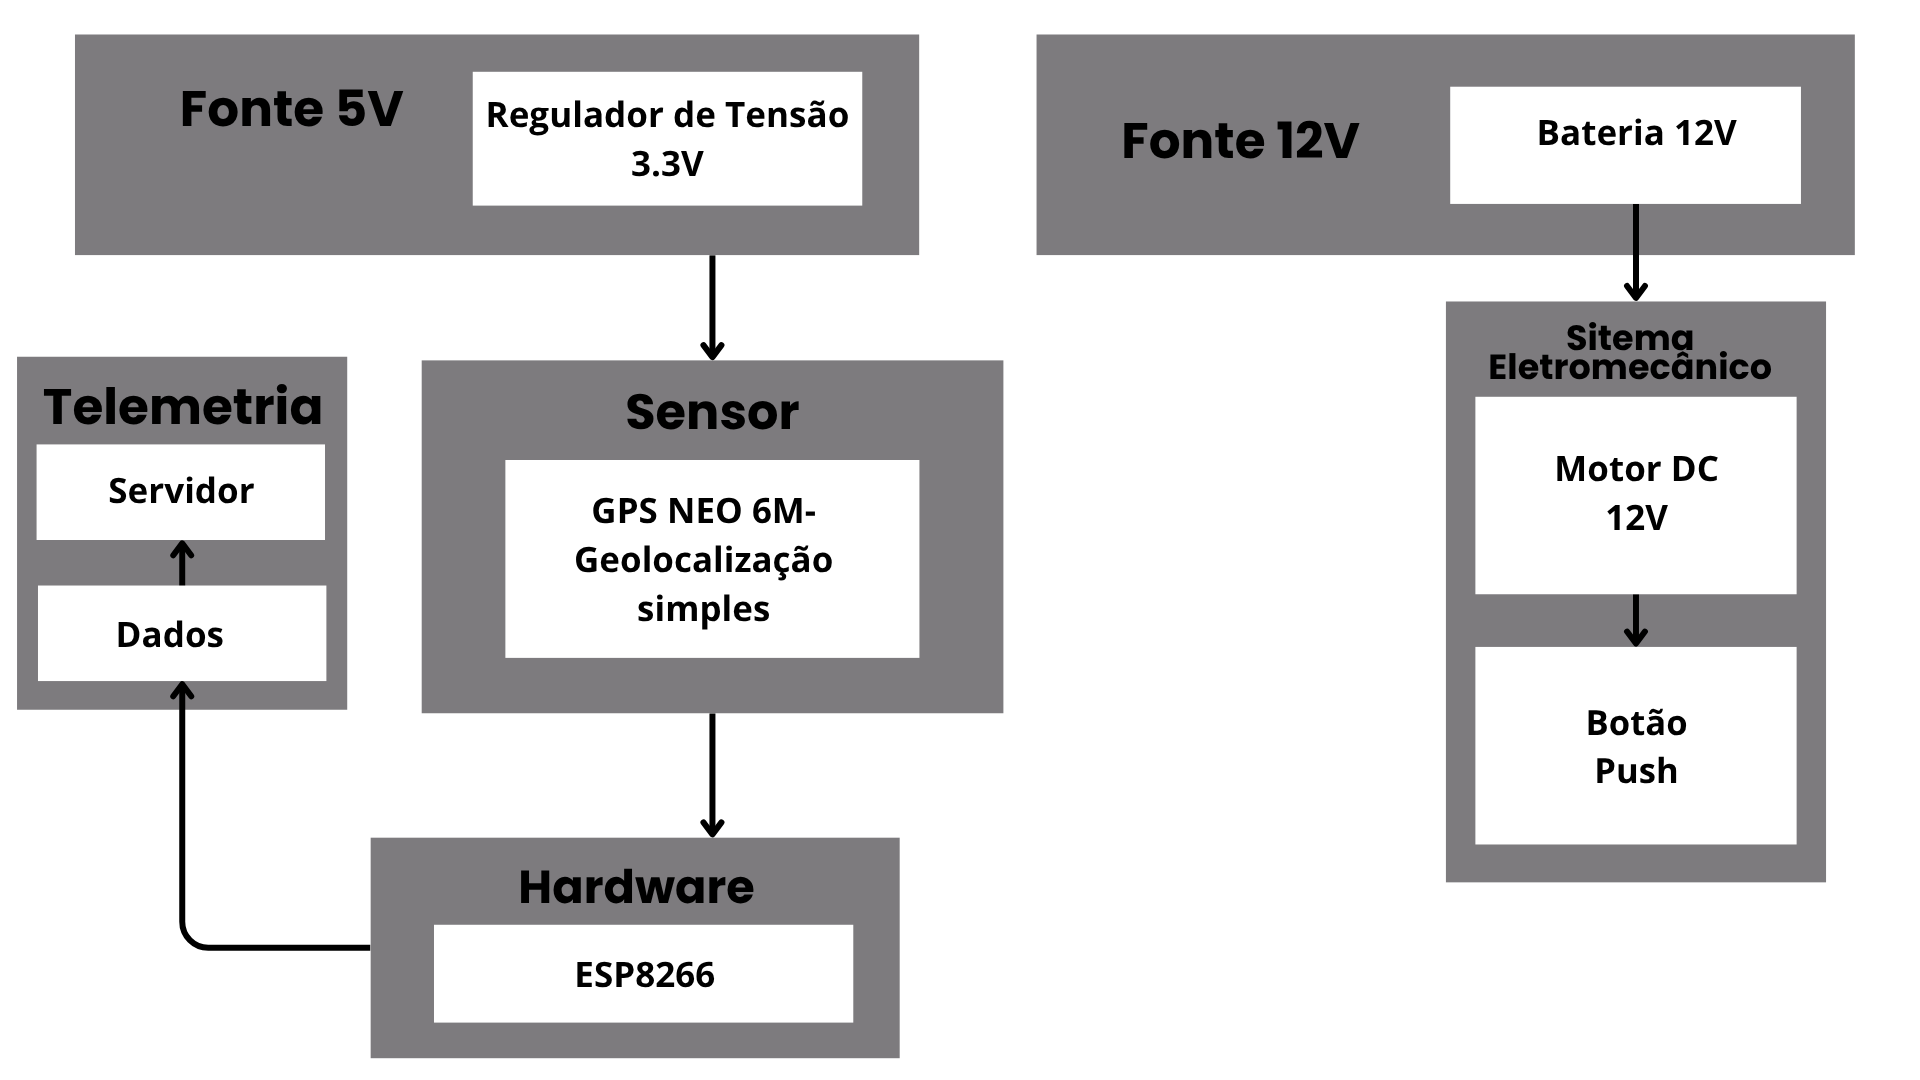
\includegraphics[width=0.6\linewidth]{figuras/ESP8266.png}
    \caption{Diagrama de blocos}
    \label{fig:diagrama de blocos}
\end{figure}

 \subsection{Esquemático elétrico para telemetria:}

 Os esquemáticos elétricos detalharão as conexões precisas entre todos os componentes de cada placa, especificando nomes, símbolos e pinagem. Para a Placa de Telemetria, o esquemático ilustra a conexão do ESP8266 (pinos de alimentação, comunicação serial com o GPS, e os pinos de controle e I/O) ao módulo GPS ATK-NEO-6M (pinos 1 para o VCC, pino 4 para o GND, pino 2 para TX, pino 3 para RX). Também contém o circuito do regulador de tensão AMS1117-3.3V, mostrando seu VIN, VOUT, GND, e os capacitores de filtro de 10µF em sua entrada e saída, o resistor de 10kΩ para fazer o pull up. Na Placa de Acionamento, o esquemático apresentará o botão K4-6x6-TH fornecendo o sinal de disparo para a base do transistor NPN BD139 através de um resistor de 470Ω. O emissor do transistor será conectado ao GND e o coletor ao motor DC12V (via conector CONN-TH-2P-P5.00), com o diodo 1N4001 em paralelo com o motor (cátodo no positivo do motor, anodo no coletor do transistor) para supressão de força contra-eletromotriz. O botão push K4-6x6-TH PTH iniciará o acionamento. Jumpers macho-fêmea, fêmea-fêmea e 15m de fio flexível 22 AWG serão utilizados para as interconexões elétricas gerais entre placas, componentes para  garantir o limite de segurança de no mínimo 5 metros de distância da equipe.


 \begin{figure}[H]
    \centering
    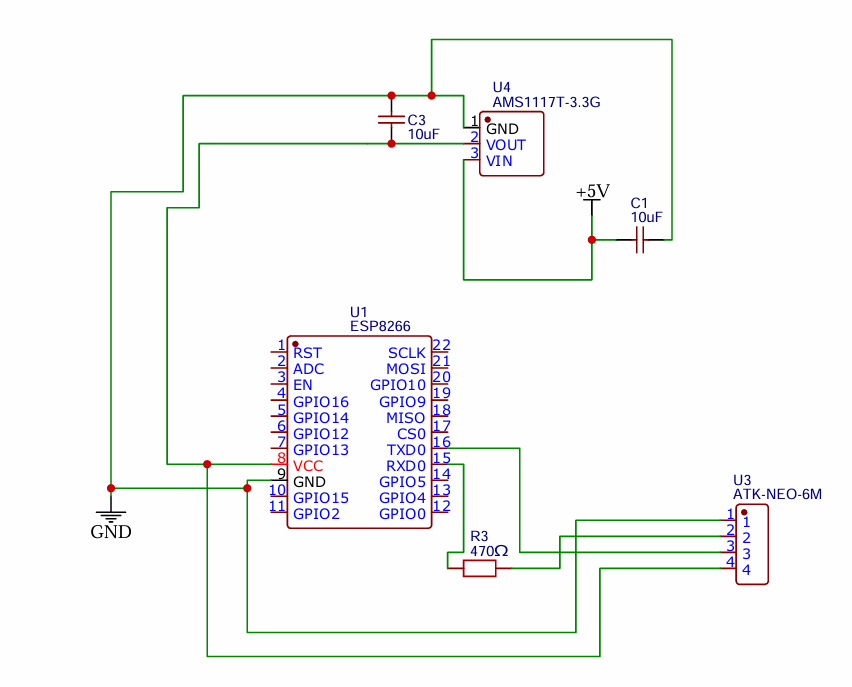
\includegraphics[width=0.5\linewidth]{figuras/esp.png}
    \caption{Esquemático elétrico para telemetria}
    \label{fig:diagrama de blocos}
\end{figure}

%\pagebreak

\begin{figure}[H]
    \centering
    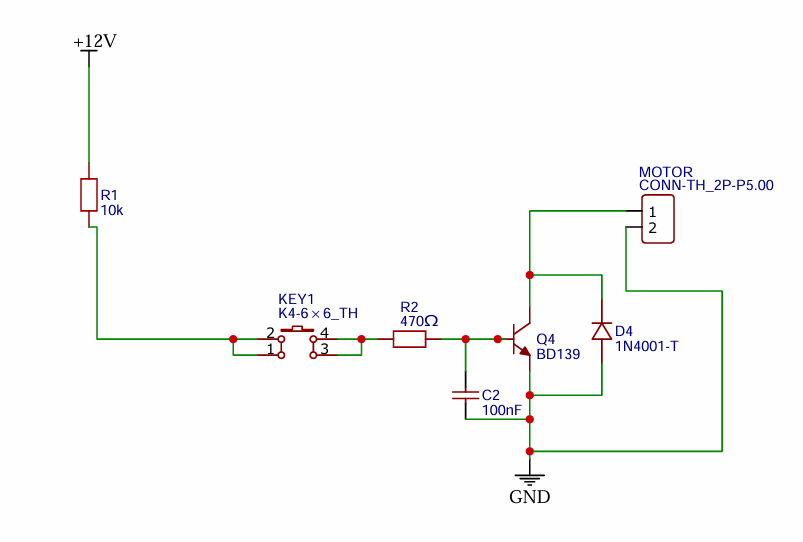
\includegraphics[width=0.5\linewidth]{figuras/motor.png}
    \caption{Esquemático para acionamento eletromecânico}
    \label{fig:diagrama de blocos}
\end{figure}

 \section{Análise de consumo energético}

Nessa seção, faremos a modelagem matemática do projeto, analisando objetivos, estrutura, movimento e trajetória. Nesse primeiro momento, ao analisar o movimento cinemático do foguete, utilizaremos a referência \cite{moyses}.

 Tendo em vista o objetivo de atingir um alcance máximo de 30 metros, definimos então que num ângulo de lançamento de 45° o foguete deve atingir os 30 metros de alcance, uma vez que esse é o ângulo de alcance máximo para o lançamento de um projétil.  Analisando as componentes vertical e horizontal do movimento do foguete, vamos encontrar o tempo necessário para que ele realize o movimento completo:
\begin{equation}
    v=v_{oy}+\frac{at}{2} \xrightarrow{} 0=v_{oy}-\frac{9,81t}{2}\xrightarrow{}v_{oy}=\frac{9,81t}{2},
    \label{componente vertical}
\end{equation}
\begin{equation}
    s=s_o+v_{ox}.t \xrightarrow{} 30=v_{ox}.t \xrightarrow{} v_{ox}=\frac{30}{t}.
    \label{componente horizontal}
\end{equation}

Note que na equação \ref{componente vertical}, o tempo t é dividido por 2, uma vez que essa componente da velocidade zera o seu valor ao chegar na altura máxima, ou seja, na metade da trajetória.

Considerando que o ângulo de lançamento para esse caso é de 45°, as componentes \(v_{ox}\) e \(v_{oy}\) são numericamente iguais, portanto:
\begin{equation}
    \frac{30}{t}=\frac{9,81t}{2} \xrightarrow{} t^2=\frac{30.2}{9,81} \xrightarrow{} t \approx 2,5s.
    \label{tempo t}
\end{equation}

A partir disso, encontramos, também, a velocidade inicial necessária do foguete:

\begin{equation}
     v_o.cos 45°=v_{ox} \xrightarrow{} v_o= \frac{v_{ox}.2}{\sqrt{2}}\xrightarrow{} v_o=\frac{\frac{30}{t}2}{\sqrt{2}} \xrightarrow{} v_o \approx 17 m/s.
     \label{vo}
\end{equation}

Agora que analisamos o movimento cinemático do projeto, partimos para a dinâmica, ou seja, tudo aquilo que causa o movimento do foguete. Para esse cálculo analítico, utilizaremos a referência \cite{rocketpropulsionelements}.
Encontramos primeiramente, a velocidade de escape da água, por meio da equação do foguete. Entretanto, são necessários os parâmetros de massa do foguete, ou seja, a massa inicial do foguete com água e a massa final dele, depois de todo o impulso dado. Para esses parâmetros faremos uma estimativa a partir dos cálculos e dados experimentais encontrados em \cite{tcc}, onde, para o nosso objetivo, a razão de massas é de aproximadamente 4. Encontramos, então, a velocidade de escape da água:
\begin{equation}
    \Delta V=v_o= v_e.\ln{\frac{m_o}{m_f}}.
    \label{ve}
\end{equation}
\begin{equation}
    v_e=\frac{\Delta V}{\ln{\frac{m_o}{m_f}}} \xrightarrow{} v_e=\frac{17}{ln{4}} \approx 12,26 m/s.
\end{equation}
Sabendo a velocidade de escape, podemos, por meio da equação de Bernoulli, considerando o fluxo ideal e incompressível e a densidade da água de 1000 \(kg/m^3\) , encontrar a pressão manométrica do foguete, ou seja, a pressão necessária dentro da cápsula de ar para o alcance da missão.

\begin{equation}
    P_o+\frac{\rho. v^2}{2}=P+\frac{\rho . v_e^2}{2} \xrightarrow{} \Delta P=\frac{\rho.v_e^2}{2} - \cancel{\frac{\rho.v^2}{2}} \xrightarrow{} \Delta P=\frac{1000.12,26^2}{2} \approx 75154 Pa.
    \label{delta P}
\end{equation}

Calculamos, então, o fluxo de massa de água, por meio de:
\begin{equation}
    \dot{m}=\rho.A.v_e
    \label{mponto}
\end{equation}
em que A é a área de saída da água. Estimando a área de saída da garrafa como aproximadamente 5 \(cm^2\), encontramos o seguinte resultado de fluxo de massa:
\begin{equation}
    \dot{m}=1000.5.10^{-4}.12,26 \approx 6,13kg/s.
\end{equation}
Calculamos então o empuxo necessário:
\begin{equation}
    T=\dot{m}.v_e=6,13.12,26=75,15N
    \label{empuxo}
\end{equation}

Por fim, baseado na teoria proposta pela referência \cite{rocketpropulsionelements}, e considerando que o "tempo de queima", ou seja, o tempo de duração que a água vai ser expelida seja 1/20 do tempo da trajetória, encontramos o impulso total necessário:
\begin{equation}
    I_t=T.\Delta t =75,15.0,125=9,39N.s
    \label{impulso total}
\end{equation}

E, finalmente, calculamos o consumo de água do foguete para um alcance de 30 metros:
\begin{equation}
    Q_{agua}=\dot{m}.t_q= 6,13.0,125=766,25mL ,
    \label{quantidade de agua}
\end{equation}
com \(t_q\) sendo o tempo de queima considerado.
Para os outros alcances, vamos variar apenas a pressão necessária no compartimento, ou seja, manteremos o ângulo de lançamento. Repetimos o processo dos cálculos para um alcance de 10 m e 20 m.


\begin{table}[h!]
\begin{tabular}{llllllllll}
Alvo & t  & $t_q$ & $v_o$   & $v_e$    & $\dot{m}$ & T & $I_t$ & $\Delta P$ & $Q_{agua}$ \\
10m     & 1,45s               & 0,0725s            & $9,75m/s$  & $7,03m/s$ & $3,52kg/s$                 & 24,75N      & 1,8N.s               & 24710,45Pa            & 0,2552L               \\
20m     & 2,04s               & 0,102s            & $13,86m/s$ & $10m/s$ & $5kg/s$                 & 50N        & 5,1N.s               & 50000Pa            & 0,51L             
\end{tabular}
\end{table}


Foi feito o mesmo passo a passo das contas feitas para um alcance de 30 metros, utilizando as seguintes equações: equação \ref{tempo t} para o tempo t, equação \ref{vo} para o \(v_o\), equação \ref{ve} para o cálculo do \(v_e\), equação \ref{mponto} para o cálculo do \(\dot{m}\), equação \ref{empuxo} para o cálculo de T, equação \ref{impulso total} para o cálculo do \(I_t\), equação \ref{delta P} para o cálculo do \(\Delta P\) e, por fim, equação \ref{quantidade de agua} para o cálculo do \(Q_{agua}\).

 Para garantir o funcionamento eficiente do sistema eletrônico no foguete de água, é fundamental realizar uma análise do consumo energético. 	Como o projeto envolve diversos componentes eletrônicos com exigências distintas de tensão e corrente, será utilizado um regulador de tensão. Esse dispositivo permitirá adaptar a tensão fornecida pela bateria às necessidades específicas de cada parte do circuito, assegurando a integridade e o desempenho ideal. 

 Para  analisar a potência consumida em cada componente individualmente, será considerado o consumo médio da corrente e a tensão ideal. A forma utilizada para o cálculo é:
 \begin{equation}
     P = V \cdot I 
 \end{equation}

 onde P é a potência (em watts), V é a tensão (em volts), e I a corrente elétrica (em amperes)

 A partir dos dados obtidos, será possível estimar o consumo total do sistema e, com isso, selecionar uma bateria que ofereça a tensão adequada e capacidade suficiente para garantir a autonomia e o funcionamento seguro durante toda a operação do foguete.

\begin{landscape}
    \begin{table}[]
\begin{center}
\caption{Comparação entre baterias}
\begin{tabular}{|l|c|c|c|c|c|}
\hline
\multicolumn{1}{|c|}{\textbf{Componentes}}                       & \textbf{\begin{tabular}[c]{@{}c@{}}Tensão \\ Operação (V)\end{tabular}} & \textbf{Corrente (A)} & \textbf{\begin{tabular}[c]{@{}c@{}}Regulador \\ necessário\end{tabular}} & \textbf{Tipo de regulador}                                           & \textbf{Observações}                                                                      \\ \hline
Bateria                                                          & 5                                                                       & 5 (máx)               & -                                                                        & -                                                                    & Fonte primária                                                                            \\ \hline
Solenoide                                                        & 12                                                                      & 1.0-2.0               & Não                                                                      & -                                                                    & \begin{tabular}[c]{@{}c@{}}Alimentação direta \\ na bateria\end{tabular}                  \\ \hline
Arduino Uno                                                      & 5                                                                       & 0.05-0.1              & Sim                                                                      & \begin{tabular}[c]{@{}c@{}}LM2596 (Buck 12V \\ para 5V)\end{tabular} & Evita superaquecimento                                                                    \\ \hline
\begin{tabular}[c]{@{}l@{}}Módulo GPS \\ (GY-NEO7M)\end{tabular} & 5                                                                       & 0.1                   & Sim                                                                      & \begin{tabular}[c]{@{}c@{}}LM2596 (Buck 12V \\ para 5V)\end{tabular} & \begin{tabular}[c]{@{}c@{}}Compartilha a mesma \\ linha\end{tabular}                      \\ \hline
Sensor MPU6050                                                   & 3,3                                                                     & 0.003                 & Sim                                                                      & AMS1117 - 3,3V                                                       & \begin{tabular}[c]{@{}c@{}}Alimentado a partir do \\ 5V regulado\end{tabular}             \\ \hline
Sensor BMP280                                                    & 3,3                                                                     & 0.002                 & Sim                                                                      & AMS1117 - 3,3V                                                       & \begin{tabular}[c]{@{}c@{}}Pode compartilhar o mesmo \\ regulador do MPU6050\end{tabular} \\ \hline
Módulo SD Card                                                   & 5                                                                       & 0.05                  & Sim                                                                      & \begin{tabular}[c]{@{}c@{}}LM2596 (Buck 12V \\ para 5V)\end{tabular} & -                                                                                         \\ \hline
\end{tabular}
\end{center}
\end{table}
\end{landscape}

 %\begin{figure}[H]
     %\centering
     %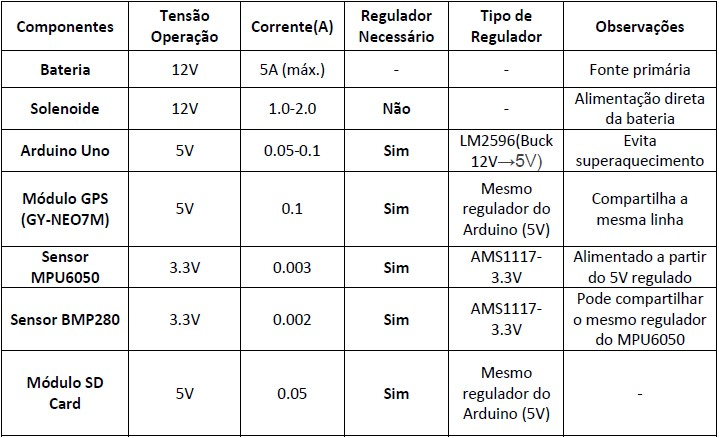
\includegraphics[width=0.75\textwidth]{figuras/Tabela.jpg}
   % \caption{Tabela}
    % \label{fig:tabela}
% \end{figure}

 \noindent Esquema de Conexões:

 \begin{figure}[H]
     \centering
     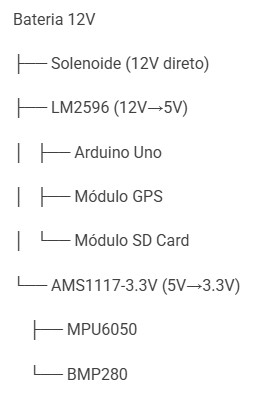
\includegraphics[width=0.3\textwidth]{figuras/Esquema.jpg}    
     \caption{Esquema de conexões}
     \label{fig:tabela}
 \end{figure}


 \noindent Cálculo de autonomia:
 \begin{itemize}
     \item Energia da Bateria
     \item $5V \cdot5Ah = 25 Wh (90.000J)$ - Bateria do Foguete
     \item $12V \cdot5Ah = 60 Wh (216.000J)$ - Bateria de acionamento do Foguete
     \item Consumo por lançamento: ~242J (incluindo solenoide)
     \item Lançamentos possíveis:
     \subsubitem 90.000J/242J/lançamento = 371,90 $\approx$ 371 lançamentos
     \subsubitem 216.000J/242J/lançamento = 216.000 $\approx$ 892 lançamentos
 \end{itemize}
 

 \begin{landscape}
\section{Descrição de \textit{software}}
\subsection{Diagrama BPMN}

O BPMN é uma notação que oferece modelos e representações gráficas para visualizar de forma clara os fluxos de atividades e as etapas dos processos dentro de ambientes empresariais e projetos. Seu principal foco é fornecer diagramas de fácil compreensão para todas as pessoas envolvidas, garantindo que todos os membros do grupo estejam alinhados aos objetivos do projeto.

\begin{figure}[H]
    \centering
    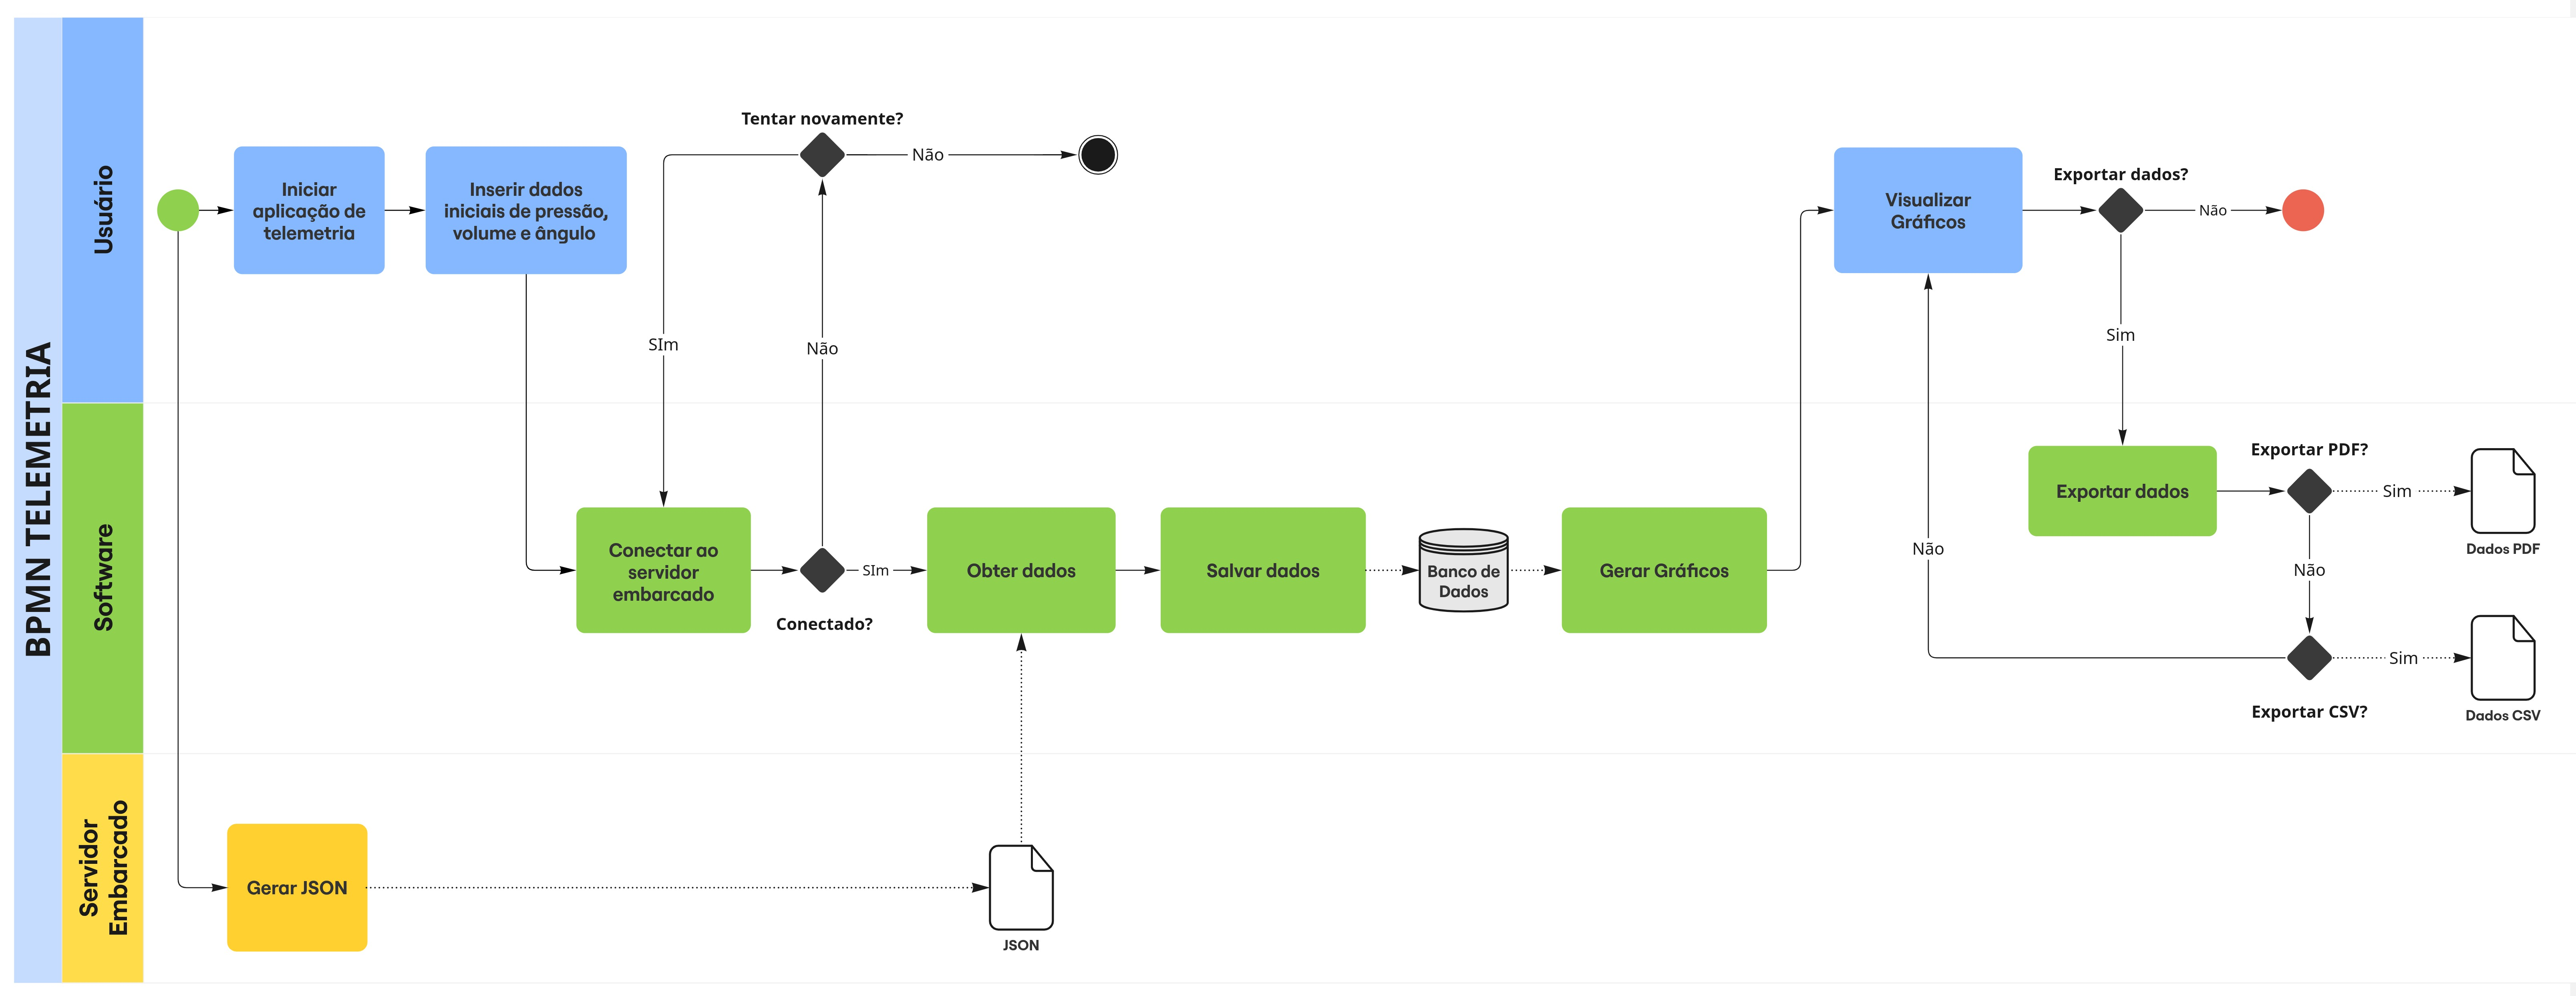
\includegraphics[width=1\linewidth]{editaveis/figuras/bpmn.jpg}
    \caption{Diagrama BPMN}
    \label{fig:enter-label}
\end{figure}
\end{landscape}

\subsection{Backlog Funcional}
O backlog funcional é uma lista organizada de funcionalidades que um sistema deve implementar para atender às necessidades dos usuários. Ele serve como um guia para o desenvolvimento do software, definindo o que precisa ser feito, por que e para quem.

O backlog funcional do projeto Oásis segue o formato de histórias de usuário, representando os requisitos funcionais sob a perspectiva do usuário final. Elas seguem um formato padrão:

\textit{“Eu, como [tipo de usuário], quero [ação] para [benefício].”}

Esse formato ajudará a equipe de software a entender quem vai usar a funcionalidade, o que a pessoa deseja fazer e por que tal funcionalidade é importante.

Os requisitos funcionas foram classificados utilizando o MoSCoW, técnica utilizada para definir a prioridade de cada funcionalidade no backlog.

O operador representa a pessoa que utilizará diretamente o sistema.

\setlength{\extrarowheight}{2pt}

% --- PARTE 1 DA TABELA 4 ---
\begin{table}[H] 
    \caption{Backlog Funcional.}
    \label{tab:backlog_funcional}
    \hfill\textit{(Continua)}
    
    \centering
    \begin{tabular}{|p{2.5cm}|p{3.5cm}|l|p{5.5cm}|c|}
    \hline
    \textbf{Épico} & \textbf{Feature} & \textbf{ID} & \textbf{História de Usuário} & \textbf{MoSCoW} \\
    \hline
    E01 Coleta de Telemetria & F01: Conexão ao servidor embarcado & US01 & Eu, como operador, quero conectar o software ao servidor embarcado no foguete para iniciar a leitura dos dados de voo. & Must \\
    \cline{2-5}
    & F02: Requisição de dados JSON & US02 & Eu, como operador, quero requisitar os dados do voo em formato JSON para processá-los no sistema. & Must \\
    \cline{2-5}
    & F03: Persistência dos dados & US03 & Eu, como operador, quero salvar os dados coletados em um banco de dados para uso posterior e comparação entre lançamentos. & Must \\
    \hline
    E02 Análise de Voo & F04: Visualização gráfica & US04 & Eu, como operador, quero visualizar gráficos de aceleração e velocidade para analisar a trajetória do foguete. & Must \\
    \hline
    \end{tabular}
\end{table}

% --- PARTE 2 DA TABELA 4 (CORRIGIDO) ---
\begin{table}[H] 
    % Título manual centralizado
    \centerline{\textbf{Tabela 4 – Backlog Funcional.}}
    % Marcador de conclusão alinhado à direita
    \hfill\textit{(Conclusão)}
    
    \vspace{0.1cm} % Pequeno espaço vertical
    \centering
    \begin{tabular}{|p{2.5cm}|p{3.5cm}|l|p{5.5cm}|c|}
    \hline
    \textbf{Épico} & \textbf{Feature} & \textbf{ID} & \textbf{História de Usuário} & \textbf{MoSCoW} \\
    \hline
    % Note que a primeira coluna (Épico) fica vazia para as features do E02
    & F05: Indicadores de desempenho & US05 & Eu, como operador, quero ver o tempo de voo e distância final para verificar se os requisitos de alcance foram atendidos. & Should \\
    \cline{2-5}
    & F06: Análise comparativa & US06 & Eu, como operador, quero comparar os dados entre os três lançamentos para calibrar o foguete com base nos resultados. & Could \\
    \hline
    E03 Interface com o Usuário & F07: Dashboard interativo & US07 & Eu, como operador, quero navegar entre as telas de conexão, gráficos e análise para usar o sistema com facilidade. & Should \\
    \cline{2-5}
    & F08: Exportação dos dados & US08 & Eu, como operador, quero exportar os dados dos lançamentos em CSV para realizar análises externas. & Could \\
    \cline{2-5}
    & F09: Exportar relatório em PDF & US09 & Eu, como operador, quero exportar os gráficos e dados em formato .PDF para documentar o desempenho do foguete. & Could \\
    \hline
    E04 Calibração de Trajetória & F10: Ajuste por parâmetros & US10 & Eu, como operador, quero visualizar os dados de entrada como pressão, volume e ângulo para entender seu impacto no desempenho. & Should \\
    \hline
    \end{tabular}
\end{table}





\renewcommand{\arraystretch}{1.2} % Espaçamento entre linhas

\subsection{Backlog Não-Funcional}

O \textbf{Backlog Não-Funcional} reúne os requisitos que não dizem respeito diretamente às funcionalidades do sistema, mas que garantem sua qualidade, desempenho, segurança, usabilidade e outros atributos essenciais. Esses requisitos asseguram que o sistema funcione de maneira eficaz, seja confiável, seguro, escalável e mantenha a integridade dos dados e da experiência dos usuários.



% --- PARTE 1 DA TABELA 5 ---
\begin{table}[H]
    \caption{Backlog Não-Funcional.}
    \label{tab:backlog_nao_funcional}
    \hfill\textit{(Continua)}

    \centering
    \begin{tabular}{|p{5cm}|p{3cm}|p{6cm}|}
        \hline
        \textbf{Requisito} & \textbf{Tipo} & \textbf{Justificativa} \\
        \hline
        O sistema deve registrar e armazenar dados de lançamento em até 2 segundos após a coleta & Desempenho & Garante tempo real para análise e resposta dos dados coletados \\
        \hline
        A base de dados deve persistir os dados de cada lançamento com 100\% de integridade & Confiabilidade & Evita perda de dados críticos para análise e calibração \\
        \hline
        A interface de análise de dados deve funcionar em desktops e notebooks das equipes & Usabilidade & Permite acesso ao sistema com os dispositivos disponíveis no ambiente escolar \\
        \hline
        O sistema deve proteger contra alterações manuais nos dados armazenados & Segurança & Garante veracidade dos dados para fins de avaliação \\
        \hline
        O software não deve depender de bibliotecas comerciais ou soluções prontas de terceiros & Legalidade & Atende às exigências do projeto pedagógico de autoria própria \\
        \hline
         O sistema deve suportar a entrada de até 3 lançamentos consecutivos por foguete & Escalabilidade & Compatível com a reutilização obrigatória dos foguetes \\
        \hline
        O tempo de carregamento das visualizações não deve ultrapassar 3 segundos com até 3 lançamentos & Desempenho & Mantém fluidez e rapidez na apresentação de dados \\
        \hline
        A plataforma de lançamento deve garantir uma zona segura mínima de 5 metros ao redor & Segurança & Protege a integridade física dos envolvidos no experimento \\
        \hline
        A coleta de dados deve ocorrer com precisão mínima de 0,1 unidade nas variáveis medidas & Precisão Técnica & Garante exatidão nas estimativas de trajetória e calibração do foguete \\
        \hline
    \end{tabular}
\end{table}

% --- PARTE 2 DA TABELA 5 (CORRIGIDO) ---
\begin{table}[H]
    \centerline{\textbf{Tabela 5 – Backlog Não-Funcional.}}
    \hfill\textit{(Conclusão)}
    
    \vspace{0.1cm}
    \centering
    \begin{tabular}{|p{5cm}|p{3cm}|p{6cm}|}
        \hline
        \textbf{Requisito} & \textbf{Tipo} & \textbf{Justificativa} \\
        \hline    
        O sistema deve ser documentado e compreensível por todos os membros das engenharias envolvidas & Manutenibilidade & Permite colaboração multidisciplinar e futuras melhorias \\
        \hline
        Os dados de posição e altitude devem ser compatíveis com os sensores integrados ao hardware & Compatibilidade & Garante integração entre software e hardware de medição \\
        \hline
        O código-fonte deve seguir boas práticas de programação e versionamento & Qualidade Técnica & Facilita auditoria, revisão por pares e evita plágios entre grupos \\
        \hline
    \end{tabular}
\end{table}

\subsection{Diagrama de Casos de Uso (UML)}

O diagrama de casos de uso tem como objetivo representar as principais funcionalidades do sistema e as interações entre os usuários (atores) e o sistema. Esse diagrama auxilia na visualização dos requisitos funcionais, permitindo um entendimento claro das funcionalidades que serão implementadas no sistema.

\begin{figure}[H]
    \centering
    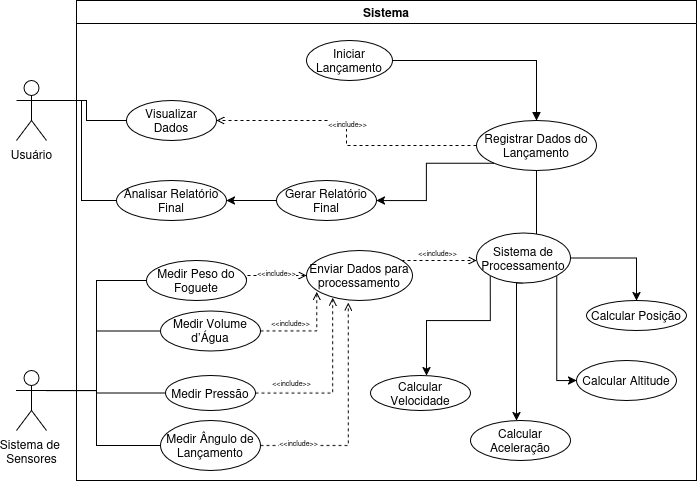
\includegraphics[width=0.75\linewidth]{editaveis/figuras/DiagramaCasoUso.png}
    \caption{Diagrama de Casos de Uso}
    \label{fig:diagrama-casos-uso}
\end{figure}

    
  \subsection{Diagrama Arquitetura}
  O diagrama de arquitetura é uma representação visual essencial no desenvolvimento de software, funcionando como um guia para estruturar e compreender um sistema. Ele oferece uma visão holística de como os componentes internos interagem entre si e com entidades externas, facilitando a comunicação entre stakeholders, apoiando decisões de design e servindo como referência para implementação e manutenção futura. Ao expor as relações entre as partes do sistema, também ajuda a identificar gargalos potenciais ou desafios de integração.

No diagrama em análise, observamos uma estrutura organizada em duas camadas fundamentais: o frontend (lado do cliente) e o backend (servidor). No frontend, a aplicação NexJs juntamente com TaliwindCSS para estilização oferece uma interface dinâmica e funcional, concentrando-se em operações CRUDs (criação, consulta, atualização e exclusão de dados) e um Dashboard para visualização e análise de informações.

No backend, o ambiente NodeJS e o framework ExpressJS estabelecem as rotas REST que viabilizam a comunicação com o Supabase, responsável pelo armazenamento e gestão de dados. Essa camada processa a lógica de negócios para entidades específicas como Lançamento, Foguete e Sensor, gerenciando suas operações CRUDs e configurando a integração com o banco de dados.

A comunicação entre as camadas ocorre exclusivamente via protocolo HTTP e APIs REST, garantindo interoperabilidade e controle de fluxo. O frontend solicita ações ao backend, que por sua vez consolida e persiste os dados no Supabase, retornando respostas para atualização da interface do usuário.

Essa arquitetura proporciona uma solução robusta e escalável para monitoramento de foguetes e sensores, onde a separação clara de responsabilidades — interface (frontend), regras de negócio (backend) e armazenamento (Supabase) — otimiza a manutenção e permite adaptações futuras. O uso de tecnologias modernas como ExpressJS e Supabase ainda agiliza o desenvolvimento e assegura a confiabilidade das operações de dados.

\begin{figure}[H]
  \centering
  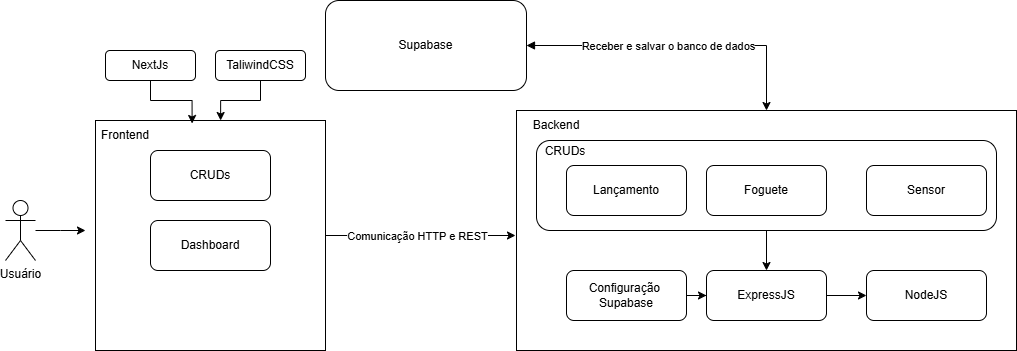
\includegraphics[width=0.9\linewidth]{editaveis/figuras/diagrama_arquitetura.png}
  \caption{Diagrama Arquitetura}
  \label{fig:enter-label}
\end{figure}



\subsection{Diagrama Entidade Relacionamento}
O DER (Diagrama Entidade-Relacionamento) é uma representação conceitual que mapeia as entidades (objetos do domínio), seus atributos e os relacionamentos, sem detalhes técnicos de implementação. No diagrama fornecido, gerado na ferramenta BrModelo, três entidades principais estruturam o modelo:

\begin{itemize}
  \item \textbf{FOGUETE} (com atributos: \textit{id, nome, peso\_ZFW}) relaciona-se com \textbf{LANÇAMENTO} através do vínculo \textit{"realiza"}, onde:
  \begin{itemize}
    \item Um foguete pode ter múltiplos lançamentos (cardinalidade 1,n);
    \item Cada lançamento pertence a um único foguete (cardinalidade 1,1).
  \end{itemize}

  \item \textbf{LANÇAMENTO} (com atributos: \textit{id, data\_hora, angulo\_inicial, nivel\_agua, pressao\_inicial, massa\_foguete\_total}) relaciona-se com \textbf{DADOCOLETADO} pelo vínculo \textit{"gera"}, onde:
  \begin{itemize}
    \item Cada lançamento produz múltiplos dados (cardinalidade 1,n);
    \item Cada dado está vinculado a um único lançamento (cardinalidade 1,1).
  \end{itemize}

  \item \textbf{DADOCOLETADO} (com atributos: \textit{id, tempo, posicoes, velocidade}) armazena as medições técnicas.
\end{itemize}

\begin{figure}[H]
\centering
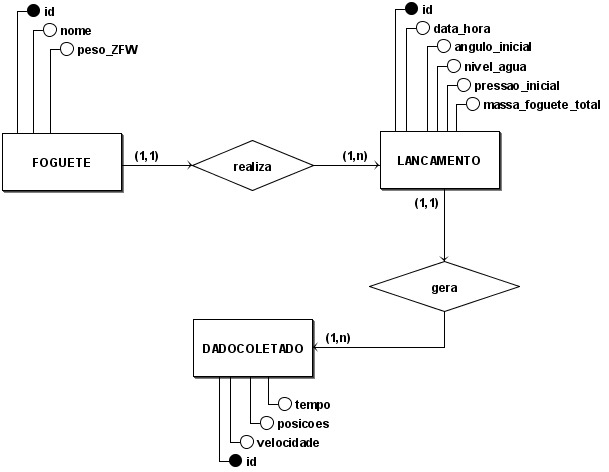
\includegraphics[width=0.5\linewidth]{editaveis/figuras/diagrama_EntidadeRelacionamento.png}
\caption{Diagrama Entidade Relacionamento}
\label{fig:enter-label}
\end{figure}

\subsection{Diagrama Lógico de Dados}

O DLD (Diagrama Lógico de Dados) é uma etapa fundamental no projeto de bancos de dados, responsável por transformar o modelo conceitual (DER) em uma estrutura técnica preparada para implementação física. Enquanto o DER foca em \textit{"o que"} o sistema precisa armazenar (entidades, atributos e relacionamentos), o DLD define \textit{"como"} esses elementos serão organizados no banco de dados, detalhando: No exemplo gerado com \textbf{BrModelo}, o DLD materializa o DER da seguinte forma:

\begin{itemize}
  \item A tabela \textbf{FOGUETE} contém os atributos: \textit{id} (UUID, chave primária), \textit{nome} (VARCHAR) e \textit{peso\_ZFW} (NUMERIC).
  
  \item A tabela \textbf{LANÇAMENTO} herda os atributos do DER e acrescenta o atributo \textit{foguete\_id} (UUID, chave estrangeira que referencia \textbf{FOGUETE}).

  \item A tabela \textbf{DADOCOLETADO} contém os atributos \textit{id, tempo, posicoes, velocidade} e se vincula à tabela \textbf{LANÇAMENTO} por meio da chave estrangeira \textit{lancamento\_id}.
\end{itemize}

\textbf{Implementação dos Relacionamentos:}
\begin{itemize}
  \item A relação \textit{"um foguete realiza múltiplos lançamentos"} (1,n) é representada pela chave estrangeira \textit{foguete\_id} na tabela \textbf{LANÇAMENTO}.

  \item A relação \textit{"um lançamento gera múltiplos dados"} (1,n) é representada pela chave estrangeira \textit{lancamento\_id} na tabela \textbf{DADOCOLETADO}.
\end{itemize}

\begin{figure}[H]
\centering
\includegraphics[width=0.75\linewidth]{editaveis/figuras/diagrama_LogicoDados.png}
\caption{Diagrama Lógico de Dados}
\label{fig:dld}
\end{figure}


\renewcommand{\arraystretch}{1.2}

Dicionário de Dados - Projeto Oásis

\subsubsection*{Entidade: FOGUETE}    

\begin{longtable}{|p{2.5cm}|p{3.5cm}|p{2cm}|p{1.8cm}|p{4cm}|}
\caption{Contém informações dos foguetes utilizados nos lançamentos}
\hline
\textbf{Atributo} & \textbf{Propriedades do Atributo} & \textbf{Tipo de Dado} & \textbf{Tamanho} & \textbf{Descrição} \\
\hline
\endfirsthead

\hline
\textbf{Atributo} & \textbf{Propriedades do Atributo} & \textbf{Tipo de Dado} & \textbf{Tamanho} & \textbf{Descrição} \\
\hline
\endhead

id & Chave primária, obrigatório & UUID & - & Identificador do foguete \\
\hline
nome & Obrigatório & VARCHAR & - & Nome do foguete \\
\hline
peso\_ZFW & Obrigatório & NUMERIC & 10,2 & Peso do foguete sem água (Zero Fuel Weight) \\
\hline
\end{longtable}

\subsubsection*{Entidade: LANCAMENTO}    

\begin{longtable}{|p{3.7cm}|p{2.7cm}|p{2cm}|p{1.8cm}|p{4cm}|}
\caption{Contém os dados relacionados aos lançamentos de foguetes com água}
\hline
\textbf{Atributo} & \textbf{Propriedades do Atributo} & \textbf{Tipo de Dado} & \textbf{Tamanho} & \textbf{Descrição} \\
\hline
\endfirsthead

\hline
\textbf{Atributo} & \textbf{Propriedades do Atributo} & \textbf{Tipo de Dado} & \textbf{Tamanho} & \textbf{Descrição} \\
\hline
\endhead

id & Chave primária, obrigatório & UUID & 11 & Identificador do lançamento \\
\hline
data\_hora & Obrigatório & DATE & - & Data e hora do lançamento \\
\hline
angulo\_inicial & Obrigatório & REAL & 2 & Ângulo inicial do lançamento \\
\hline
nivel\_agua & Obrigatório & NUMERIC & 300 & Nível de água no momento do lançamento \\
\hline
pressao\_inicial & Obrigatório & REAL & 4 & Pressão inicial no lançamento \\
\hline
massa\_foguete\_total & Obrigatório & NUMERIC & 10,2 & Massa total do foguete \\
\hline
FOGUETE\_id & Chave estrangeira, obrigatório & UUID & - & ID do foguete utilizado no lançamento \\
\hline
\end{longtable}

\subsubsection*{Entidade: DADOCOLETADO}   

\begin{longtable}{|p{3.7cm}|p{2.7cm}|p{1.6cm}|p{1.8cm}|p{4cm}|}
\caption{Contém os dados registrados durante o lançamento de um foguete}
\hline
\textbf{Atributo} & \textbf{Propriedades do Atributo} & \textbf{Tipo de Dado} & \textbf{Tamanho} & \textbf{Descrição} \\
\hline
\endfirsthead

\hline
\textbf{Atributo} & \textbf{Propriedades do Atributo} & \textbf{Tipo de Dado} & \textbf{Tamanho} & \textbf{Descrição} \\
\hline
\endhead

id & Chave primária, obrigatório & UUID & - & Identificador do dado coletado \\
\hline
LANCAMENTO\_id & Chave estrangeira, obrigatório & UUID & - & ID do lançamento ao qual os dados pertencem \\
\hline
posicoes & Obrigatório & REAL & - & Posição registrada durante o voo \\
\hline
velocidade & Obrigatório & REAL & - & Velocidade registrada durante o voo \\
\hline
tempo & Obrigatório & REAL & - & Tempo registrado correspondente aos dados \\
\hline
\end{longtable}


\subsection{Diagrama de Estados}
O diagrama de estados é um tipo de diagrama utilizado para modelar o comportamento dinâmico de um sistema, descrevendo os diferentes estados que um objeto ou sistema pode assumir ao longo do tempo, bem como os eventos ou condições que causam as transições entre esses estados.

\begin{landscape}
\begin{figure}
    \centering
    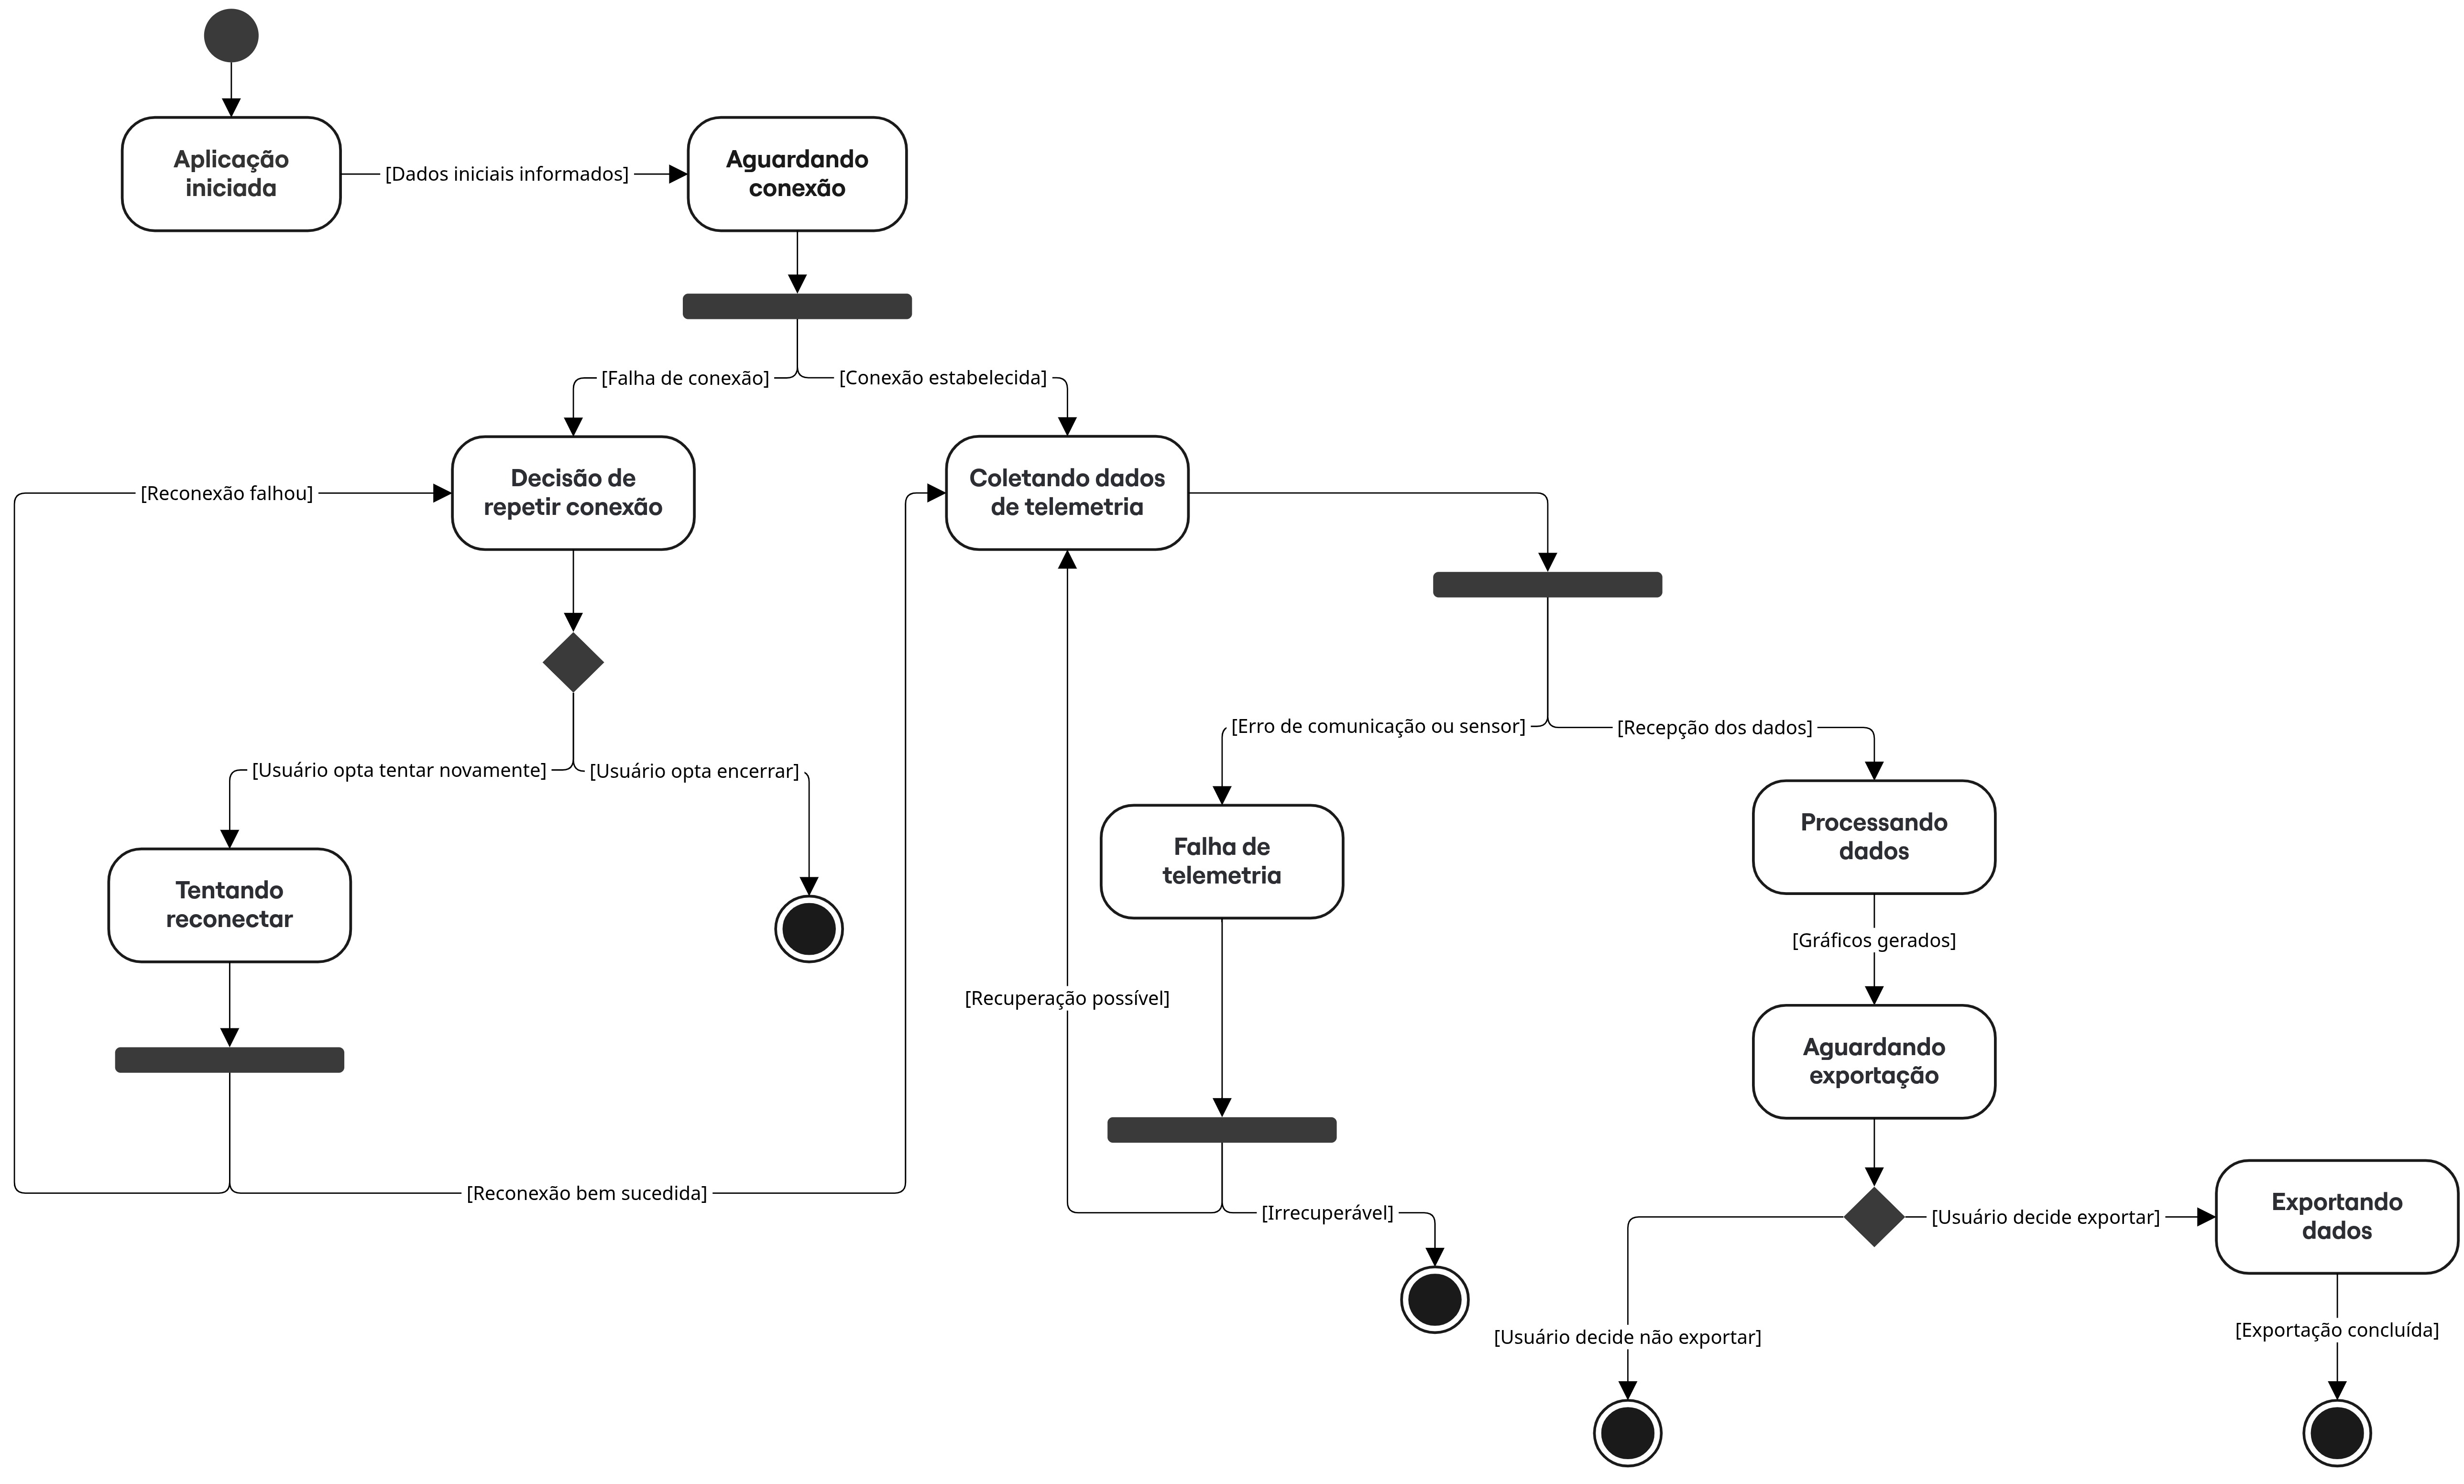
\includegraphics[width=1\linewidth]{editaveis/figuras/diagrama_de_estados.jpg}
    \caption{Diagrama de Estados}
    \label{fig:enter-label}
\end{figure}
\end{landscape}


\subsection{Protótipo funcional e navegável do software.}
Segue o link para o protótipo navegável: \href{https://www.figma.com/proto/EvktcpudU3xVgz8JVLDw5m/O%C3%A1sis-Prot%C3%B3tipo?node-id=1-2&t=MGDfspVva3MgOo6H-1&scaling=min-zoom&content-scaling=fixed&page-id=0%3A1&starting-point-node-id=1%3A2}{Protótipo}


\subsection{Especificações de Caso de Testes}

Os testes de software são fundamentais para assegurar a qualidade e a confiabilidade dos sistemas, atuando como uma barreira crítica contra falhas. Essa prática consiste em executar o programa com o objetivo explícito de identificar erros e verificar se seu comportamento está alinhado aos requisitos especificados. Além de detectar defeitos existentes, os testes ajudam a prevenir problemas futuros, conferindo maior segurança quanto à estabilidade e funcionalidade do produto final.

A especificação de testes formaliza esse processo ao estruturar os cenários de validação em um roteiro claro e sistemático. Ela define as condições de execução, os passos a serem seguidos, as entradas e os resultados esperados para cada caso, servindo como base para avaliar a conformidade com os requisitos do usuário. Para isso, utiliza-se uma tabela de casos de teste, que organiza cada cenário por meio de colunas como ID (identificador único do caso de teste, que permite rastreamento e referência rápida), Objetivo do Teste (descrição clara do que se pretende validar), Pré-condições (estado necessário do sistema antes da execução), Entradas (valores ou ações fornecidos ao sistema), Passos (sequência de ações a serem realizadas), Resultado Esperado (comportamento ou saída que o sistema deve apresentar) e Prioridade (grau de importância do teste, que auxilia na organização da execução). Essa estrutura organizada garante rastreabilidade, cobertura abrangente dos requisitos e validação minuciosa das funcionalidades — elementos essenciais para assegurar a qualidade e a confiabilidade do resultado final.


% A fonte precisa ser bem pequena para caber em modo retrato
\tiny 

% --- PARTE 1 DA TABELA 9 ---
\begin{table}[H]
    \caption{Tabela de Especificação de Casos de Teste - Software.}
    \label{tab:casos_de_teste}
    \hfill\textit{(Continua)}
    
    \centering
    \renewcommand{\theadfont}{\bfseries}
    \begin{tabular}{|p{0.8cm}|p{1.8cm}|p{1.8cm}|p{1.8cm}|p{2.3cm}|p{2.5cm}|p{1.1cm}|p{1.7cm}|}
    \hline
    \textbf{ID} & \textbf{Objetivo do Teste} & \textbf{Pré-condições} & \textbf{Entrada} & \textbf{Passos} & \textbf{Resultado Esperado} & \textbf{Prio-ridade } & \textbf{Tipo de Teste} \\
    \hline
    CT01  & Verificar inicialização da aplicação & Sistema instalado & Nenhuma & Iniciar o sistema & Tela inicial da aplicação é exibida & Alta & Teste de Sistema \\
    \hline
    CT02  & Validar entrada de dados iniciais & Aplicação iniciada & Pressão, volume e ângulo & Inserir dados e confirmar entrada & Dados são aceitos e armazenados & Alta & Teste de Sistema \\
    \hline
    \end{tabular}
\end{table}

\begin{landscape}

% --- PARTE 2 DA TABELA 9 ---
\begin{table}[H]
    \centerline{\textbf{Tabela 9 – Tabela de Especificação de Casos de Teste - Software.}}
    \hfill\textit{(Continua)}
    
    \vspace{0.1cm}
    \centering
    \renewcommand{\theadfont}{\bfseries}
    \begin{tabular}{|p{1.0cm}|p{2.5cm}|p{2.5cm}|p{2.5cm}|p{3.2cm}|p{3.0cm}|p{2.2cm}|p{2cm}|}
    \hline
    \thead{ID} & \thead{Objetivo\\do Teste} & \thead{Pré-\\condições} & \thead{Entrada} & \thead{Passos} & \thead{Resultado\\Esperado} & \thead{Prioridade} & \thead{Tipo de\\Teste} \\
    \hline
    CT03 & Verificar conexão com servidor embarcado & Dados iniciais inseridos & Nenhuma & Clicar em conectar e aguardar resposta & Sistema conecta ao servidor e exibe confirmação & Alta & Teste de Integração \\
    \hline
    CT04 & Testar reconexão após falha & Conexão inicial falhou & Opção de tentar novamente & Selecionar “tentar novamente” e aguardar reconexão & Reconexão realizada com sucesso ou tentativa encerrada & Média & Teste de Integração \\
    \hline
    CT05 & Validar coleta de dados & Conectado ao servidor & Nenhuma & Iniciar coleta e aguardar leitura de dados & Dados são recebidos com sucesso & Alta & Teste de Integração \\
    \hline
    CT06 & Testar falha na coleta & Conectado ao servidor & Comunicação interrompida ou erro & Iniciar coleta e simular erro & Sistema detecta falha e informa ao usuário & Alta & Teste de Integração \\
    \hline
    CT07 & Verificar salvamento de dados no banco & Dados coletados com sucesso & Nenhuma & Finalizar coleta e aguardar confirmação & Dados persistidos corretamente no banco & Alta & Teste de Integração \\
    \hline
    CT08 & Gerar gráficos com dados salvos & Dados salvos no banco & Nenhuma & Solicitar geração de gráficos & Gráficos são exibidos na tela & Alta & Teste de Sistema \\
    \hline
    \end{tabular}
\end{table}


% --- PARTE 3 DA TABELA 9 ---
\begin{table}[H]
    \centerline{\textbf{Tabela 9 – Tabela de Especificação de Casos de Teste - Software.}}
    \hfill\textit{(Conclusão)}
    
    \vspace{0.1cm}
    \centering
    \renewcommand{\theadfont}{\bfseries}
    \begin{tabular}{|p{1.0cm}|p{2.5cm}|p{2.5cm}|p{2.5cm}|p{3.2cm}|p{3.0cm}|p{2.2cm}|p{2cm}|}
    \hline
   \thead{ID} & \thead{Objetivo\\do Teste} & \thead{Pré-\\condições} & \thead{Entrada} & \thead{Passos} & \thead{Resultado\\Esperado} & \thead{Prioridade} & \thead{Tipo de\\Teste} \\
    \hline
    CT09 & Visualizar gráficos & Gráficos gerados & Nenhuma & Acessar seção de visualização & Gráficos são exibidos de forma clara & Alta & Teste de Sistema \\
    \hline
    CT10 & Exportar dados & Dados disponíveis & Seleção de tipo de exportação & Escolher “exportar dados”, selecionar formato e confirmar & Processo de exportação iniciado & Média & Teste de Sistema \\
    \hline
    CT11 & Exportar dados como PDF & Dados disponíveis & Selecionar exportação PDF & Iniciar exportação, selecionar “PDF” e confirmar & Arquivo PDF é gerado corretamente & Baixa & Teste de Sistema \\
    \hline
    CT12 & Exportar dados como CSV & Dados disponíveis & Selecionar exportação CSV & Iniciar exportação, selecionar “CSV” e confirmar & Arquivo CSV é gerado corretamente & Baixa & Teste de Sistema \\
    \hline
    \end{tabular}
\end{table}

\end{landscape}
